\documentclass{llncs}
%\usepackage[cp1250]{inputenc}
%\usepackage[utf8]{inputenc}
%\usepackage[czech]{babel}
\usepackage{graphicx}
\usepackage{tabularx}
%\usepackage{tipa}

\bibliographystyle{splncs}

\begin{filecontents}{citace.bib}
@inproceedings{kruuza2012making,
  title={Making Community and ASR Join Forces in Web Environment},
  author={Kr{\uu}za, Old{\v{r}}ich and Peterek, Nino},
  booktitle={International Conference on Text, Speech and Dialogue},
  pages={415--421},
  year={2012},
  organization={Springer}
}
\end{filecontents}



\begin{document}
\newtheorem{Definition}{Definition}
\title{ASR-Output-Correcting Webapp After 6 Years}

\author{Oldřich Krůza and Vladislav Kuboň}
\institute{Charles University in Prague\\
           Faculty of Mathematics and Physics\\
           Institute of Formal and Applied Linguistics\\
           Malostranské nám. 25, Prague, Czech Republic\\
           \{kruza,vk\}@ufal.mff.cuni.cz}

\maketitle

\begin{abstract}

This paper presents a next-generation web application that enables users to
contribute corrections to automatically acquired transcription of long speech
recordings. We describe differences from similar settings, compare our solution
with others and reflect on the development from the first, 6 years old version
in the light of the work done, lessons learned and the new technologies
available in the browser.

\end{abstract}

\section{Introduction}

In 2012\cite{kruuza2012making}, we presented a setting where a community of
users contributed corrections to automatically transcribed talks of a single
speaker. Now that the browser technologies evolved drastically and we could
observe the usage patterns and discover shortcomings of the solution at hand, we
have created a next generation of the programme. We shall describe the steps
taken and discuss their motivation and impact.

\subsection{Motivation}

Our project focuses on the collection of recordings of Karel Mako\v{n} *1912
\textdagger1993, the author of numerous books, translations and comments to
works of spiritual and religious nature, who was influenced by trances during
recurring surgery without anesthesy in the age of 6, ecstasies in the youth and
finally facing and surviving certain death in a Nazi concentration camp, after
which he experienced enlightenment. He gave talks in a narrow circle of friends
and the recordings in our care have been taken between early 70's and 1991,
spanning about 1000 hours in total.

All of his work deals more or less directly with a single topic: entering the
eternal life before the physical death. He draws mainly from the Christian
symbolism, builds up on Christian mysticism and ancient tradition of India.

Basically the meat of his teachings is systematically encompassed in his written
works, whereas the talks contain the sauce: talks tailored to the audience,
answering questions, personal experiences, behind-the-scenes to the books etc.

\section{Differences to other settings}

In our setting, we have a large spoken corpus (about 1000 hours) of a single
speaker. Our aim is to have a transcription as good as possible for the purpose
of searching and further, higher-level processing of the data. There is a pool
of people interested in the talks, who on one hand are the force we can try to
employ and on the other hand are the consumers of our effort, our target group
so to speak.

The web application should therefore combine the two purposes: 1. serve its user
with making the content available in a manner as good as possible and 2. animate
the user to give as much and as high-quality contribution as possible.

To our best knowledge, there is no other project with a comparable setting.
However, we can compare single aspects found in other applications.

\subsection{Transcribing apps}

The main differences to common transcribing software are that

\noindent
\begin{tabularx}{\textwidth}{
    @{\hspace{1.5em}}% Space for left bullet
    >{\leavevmode\llap{\textbullet~}\raggedright}% Left bullet + formatting of column
    X% Left column specification
    @{\quad\hspace{1.5em}}% Space between columns + right bullet space
    >{\leavevmode\llap{\textbullet~}\raggedright\arraybackslash}% Right bullet + formatting of column
    X% Right column specification
    @{}% No column space on right
  }
  \em{common transcription applications} & \em{our application} \\
  are optimized for the case where there is no transcription available and it
  must be acquired from scratch &
    always assumes a transcription is available \\
  allow annotation of speakers &
    assumes all utterances come from the same speaker \\
  need no quality control: the user is free to enter whatever transcription she
  pleases and the ultimate measure is her satisfaction &
    needs the transcription to be accurate because it is used as training data
    for the acoustic model \\
  use alignment on the level of phrases, if any &
    uses alignment on the level of words \\
  are user-centric: the user transcribes whatever acoustic data they choose &
    is data-centric: the whole application with all its tools and persons
    revolves around the data set \\
  assumes the user wants to transcribe &
    assume the user want to listen and possibly read along and we want to
    animate her to submit transcriptions \\
  has no shared data between users &
    must count with collisions
\end{tabularx}

We can still learn a lot from transcribing software. The ease of performing
common tasks, like pausing, resuming and rewinding is crucial for the user
experience and in effect for the amount of submissions that we receive. Also,
the way the text is displayed synchronously to the audio played has a big impact
and the approaches have a lot of space for variation.

\subsection{Wiki}

Where our application diverts from transciption software, it mostly resembles a
wiki: a community platform that serves its users including the contributors but
where the quality of the contributions is essential, while the contributor's
satisfaction alone is of little importance.

One major difference to a wiki is that wiki is creative, whereas our task is
mechanical. The user has basically no room for their own invention: providing a
different than correct transcription is seen as an error.

Major wikis have good measures for edit conflicts, which is where we could learn
some lessons. However, so far there was no need to do that because
\begin{enumerate}
\item{when we always simply take the most recent version
of a segment, the result stays consistent even if a piece from user A comes into
a larger transcription of user B;}
\item{our user base is so far limited to a small community who have no problem
coordinating with each other. We plan to expand to broader public soon though.}
\end{enumerate}

\section{Description of the web application}

The application consists of several views:
\begin{enumerate}
\item{the start page where all recordings are listed and each points to a detail
view,}
\item{the detail view, where a recording can be played back, its transcription
is displayed and can be corrected by the user,}
\item{search page, where hits to a search query are listed and point to
corresponding positions in the recordings,}
\item{static pages with general information, contact etc.}
\end{enumerate}

We shall only discuss the detail view as the others are not relevant to this
article. Figure~\ref{fig:scn1lab} shows the interface during playback.
Figure~\ref{fig:scn2lab} shows the interface while a segment is being edited.
The interface in the figures is conveniently shown in English, although in
reality it is in Czech.

\begin{figure}[htpb]
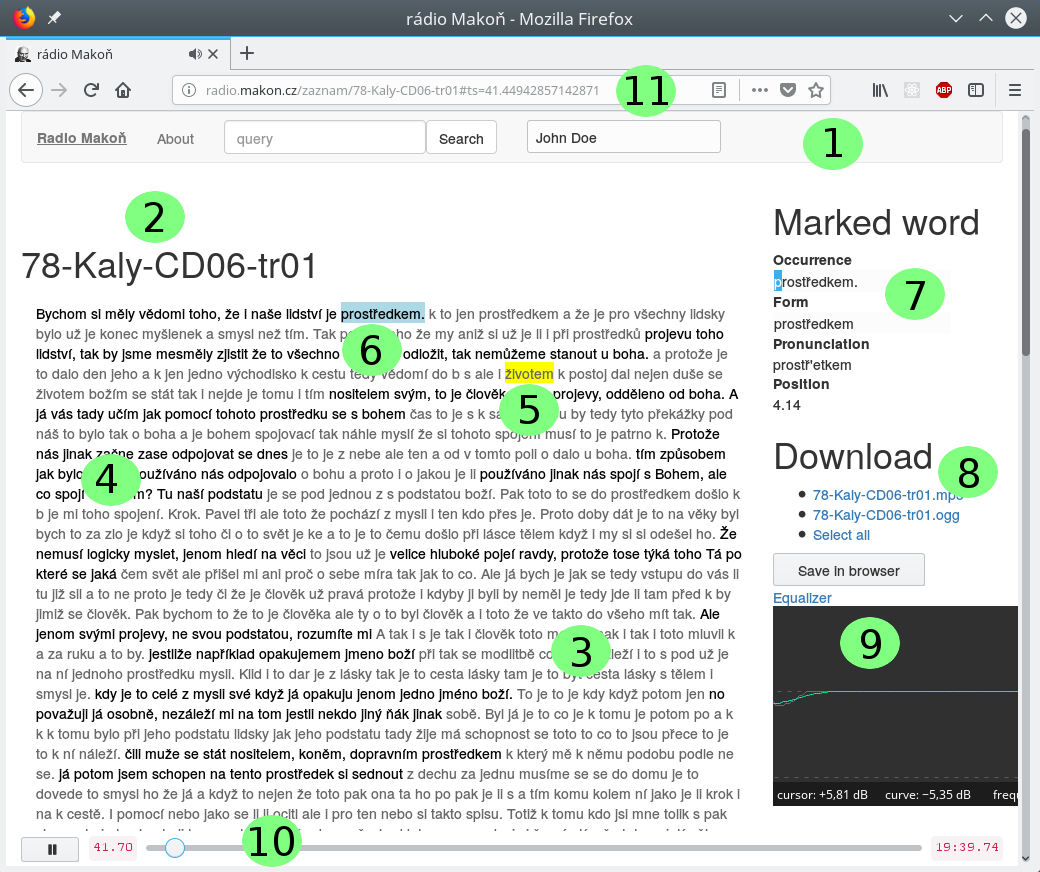
\includegraphics[scale=0.6]{rc/radio-makon-en-1-lab.png}
\caption{Web interface during playback}
\label{fig:scn1lab}
\end{figure}

Legend to Figure~\ref{fig:scn1lab}:
\begin{enumerate}
\item{
    Header with
    \begin{itemize}
    \item{app name linking to start page,}
    \item{about link,}
    \item{search field and}
    \item{username input field;}
    \end{itemize}
}
\item{Identifier of the recording;}
\item{Automatically transcribed segments in gray;}
\item{Manually transcribed segments in black;}
\item{Currently played-back word highlighted by yellow background;}
\item{Marked word highlighted in regent st. blue;}
\item{
    Marked word info:
    \begin{itemize}
    \item{
        occurrence: the word with contextual capitalization and
        punctuation as it appeard in the text, currently being edited as the
        selected initial letter reveals,
    }
    \item{form: normalized word form as it appears in the word list,}
    \item{pronunciation: Czech phonetic transcription of the word,}
    \item{
        position: time of the beginning of the word in seconds from the
        start of the recording;
    }
    \end{itemize}
}
\item{
    Tools for storing:
    \begin{itemize}
    \item{direct links to the audio files,}
    \item{selecting the whole transcription for easy pasting,}
    \item{storing the decoded recording in the browser's IndexedDB;}
    \end{itemize}
}
\item{Graphical equalizer for compensating narrow-band noise;}
\item{
    Audio playback controls:
    \begin{itemize}
    \item{play/pause button,}
    \item{current playback position,}
    \item{playback scrollbar,}
    \item{total recording length;}
    \end{itemize}
}
\item{Current position reflected in URL fragment.}
\end{enumerate}

\begin{figure}[htpb]
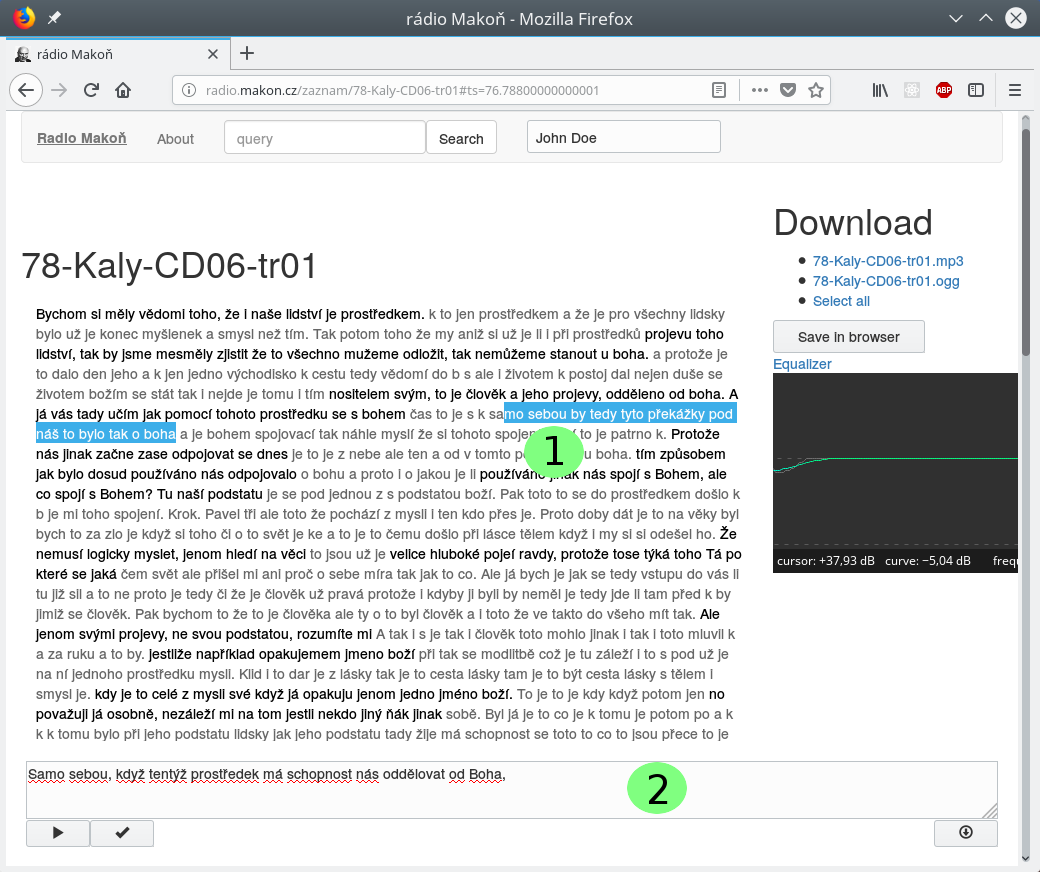
\includegraphics[scale=0.6]{rc/radio-makon-en-2-lab.png}
\caption{Interface in the state of editing a segment, with labels}
\label{fig:scn2lab}
\end{figure}

Legend to Figure~\ref{fig:scn2lab}:
\begin{enumerate}
\item{
    Selecting a text range with the mouse defines the segment the user is about
    to transcribe;
}
\item{
    The edit tool with
    \begin{itemize}
    \item{textarea prefilled with the current transcription,}
    \item{playback button that plays the corresponding segment,}
    \item{save button and}
    \item{download-segment button, which initiates a file-save action for the
    corresponding segment.}
    \end{itemize}
}
\end{enumerate}

\subsection{Displaying the transcription}

Most transcribing programs show the transcription as a vertical list of
utterances, see Figure~\ref{fig:transcriber1} for an example of
{\em{Transcriber}}\footnote{trans.sourceforge.net}, a veteran open-source
transcription tool. We attribute this to the fact that the atomic elements of
the transcription are the user-entered utterances and their boundaries are
reliable. In our case, the atomic elements are words. There are sentences, sure,
but the segmentation to sentences by the ASR is very unreliable, so we want it
to be natural to transcribe a segment overlapping sentence boundaries.

This is one of the reasons why we display the transcription basically as a
single wrapped line.

The transcription display was designed to have these features:
\begin{itemize}
\item{Currently played-back word should be highlighted;}
\item{
    Manually transcribed segments should be clearly distinct from automatically
    transcribed ones;
    \label{feats:item:manualdistinct}
}
\item{
    Selecting one or more words with the mouse should trigger transcription mode
    for the selected text;
    upon a successful save, this should be merged into the display;
}
\item{
    Clicking a word should bring up its context info (we call this the
    \em{marked word} as the term \em{selected word} is already taken);
}
\item{
    The whole transcription should be shown at once for easy searching;
    \label{feats:item:showall}
}
\item{
    The page should be responsive;\label{feats:item:speed}
}
\end{itemize}

These requirements are harder to combine than it may seem. Notably
responsiveness is hard to combine with all of the other ones. Why is that so?



\begin{figure}[htpb]
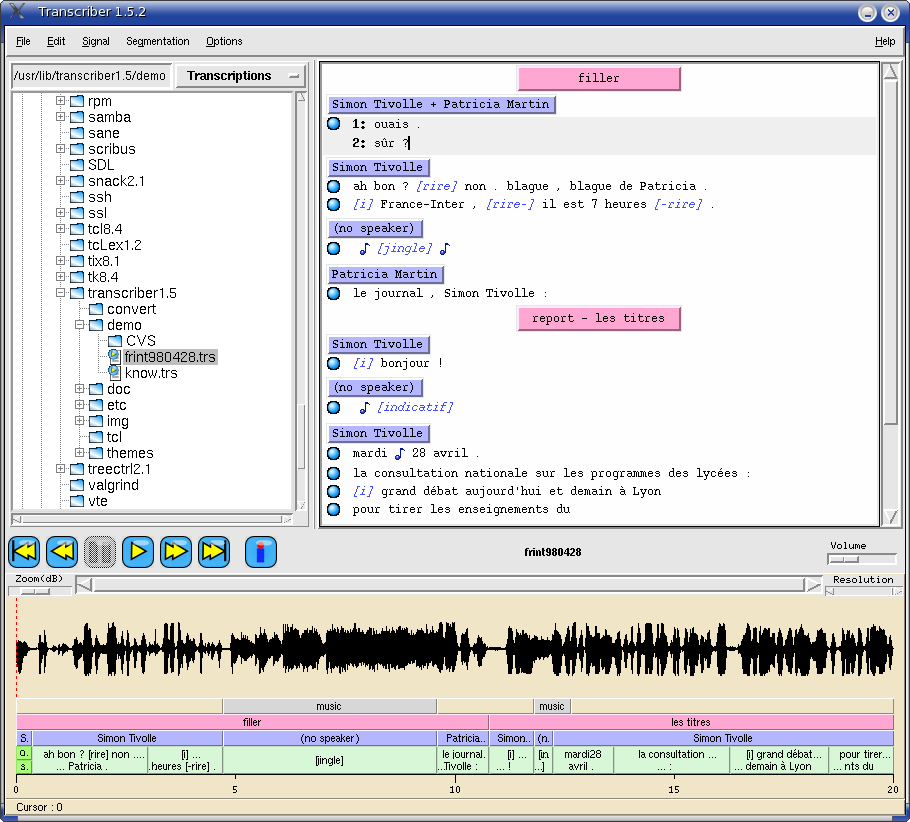
\includegraphics[scale=0.4]{rc/transcriber1.png}
\caption{A screenshot of Transcriber}
\label{fig:transcriber1}
\end{figure}

% alert when correcting humanic

%The need for quality control has wide implications. We need to perform forced
%alignment every time a segment is transcribed. Hence, it must be clear what part
%of the audio \em{exactly} the segment corresponds to. Since each word knows its
%exact timestamp, and we know which words from the old transcription are to be
%replaced, we can perform the forced alignment very precisely. This is also one
%of the reasons why our application always assumes an existing transcription.

%What concerns animating the user to provide a transcription, there must be more
%research done. The basic idea is though that when the user sees the
%transcription synchronously and it contains errors, they get the urge to fix it.

%Our first reference is
%Transcriber\footnote{sourceforge.net/projects/trans}. Transcriber is an
%open-source program written in TCL.

\section{Conclusion}

\section*{Acknowledgments}

The research was supported by SVV project number 265 314.\\
\\
This work has been using language resources stored
by the LINDAT-Clarin project of the Ministry of
Education of the Czech Republic (project LM2010013).
%\bibliography{paper}

\bibliography{citace}

\end{document}
